\documentclass[table]{beamer}
\usetheme{FAU}
\usefonttheme{FAU}
\usecolortheme{FAU}
\useinnertheme{FAU}
\useoutertheme{FAU}

\usepackage{tikz}
\usepackage{url}
\usepackage{subfigure}
\usepackage{booktabs}
\usepackage{multirow}
\usepackage{pgfplots}
\usepackage{pgfplotstable}

\setbeamerfont{caption}{size=\footnotesize}
\setbeamertemplate{caption}{\raggedright\insertcaption\par}

\newcommand{\goboard}{
	\definecolor{boardcolor}{RGB}{220,179,92}
	\draw [fill=boardcolor,black,thick] (1,1) rectangle (11,11);

	\foreach \x in {0,...,8} {
		\draw[very thick] (2+\x, 2) -- (2+\x, 10) {}; %horizontal
		\draw[very thick] (2, 2+\x) -- (10, 2+\x) {}; %vertikal
	};
}
\newcommand{\piece}[3]{\draw[fill=#1, draw=white!50!black, thick] (#2+1, #3+1) circle (0.5);}
\newcommand{\wpiece}[2]{\piece{white}{#1}{#2}}
\newcommand{\bpiece}[2]{\piece{black}{#1}{#2}}

\title[BT Presentation]{Bachelor Thesis Presentation}
\subtitle{Implementation of an Android app for the recording of Go games by tracking their state}

\institute{Pattern Recognition Lab (CS 5)}

\author{Tilman \textsc{Adler}}
\begin{document}

\frame[plain]{\titlepage}

\frame[squeeze]{\tableofcontents}

\section{Motivation}
\begin{frame}{A Really Short Introduction to Go}

	\begin{columns}
		\begin{column}{0.6\textwidth}
			\begin{itemize}
				\item This is a 9x9 Go board (there's also 11x11, 13x13 and 19x19)
				\visible<2->{\item Players alternately put pieces on the intersections}
				\visible<6->{\item The player with the most area wins}
				%\visible<7->{\item \color{gray}Plus: Pieces can be captured, not all moves are allowed}
			\end{itemize}
		\end{column}

		\begin{column}{0.4\textwidth}
			\begin{figure}
				\resizebox{\columnwidth}{\columnwidth}{%
					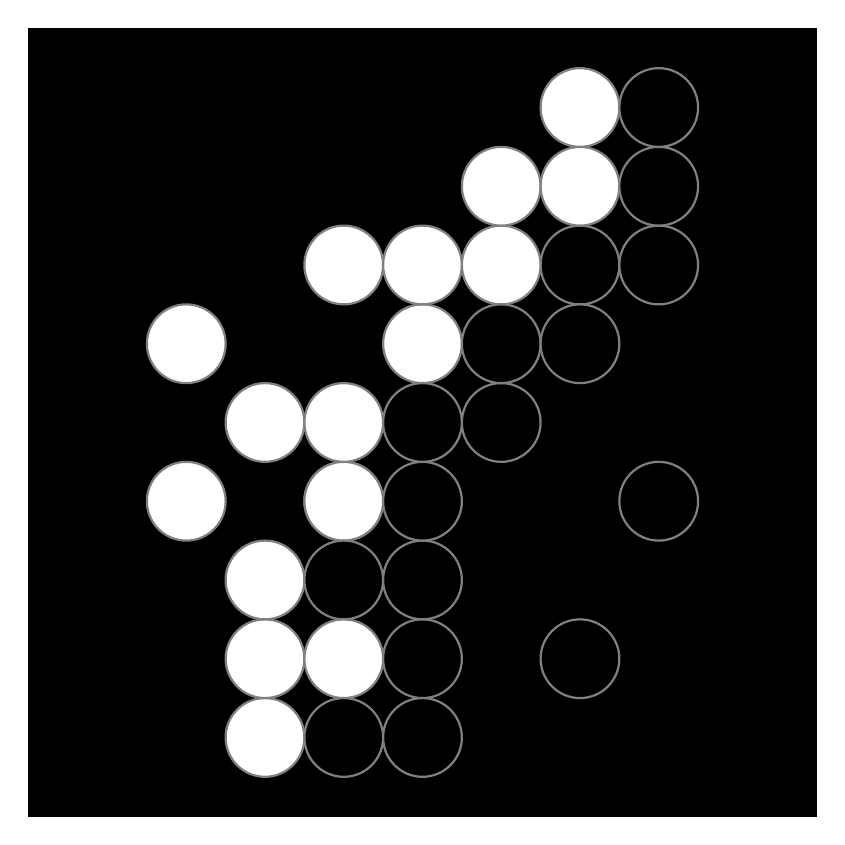
\begin{tikzpicture}[x=1cm, y=1cm]
						\goboard;

						\visible<2->{\wpiece{4}{4};}
						\visible<3->{\bpiece{7}{7};}
						\visible<4->{\wpiece{4}{7};}
						\visible<5->{\bpiece{6}{5};}
						\visible<6->{
							\wpiece{2}{6};\wpiece{2}{4};
							\wpiece{3}{1};\wpiece{3}{2};\wpiece{3}{3};\wpiece{3}{5};
							\wpiece{4}{2};\wpiece{4}{4};\wpiece{4}{5};
							\wpiece{5}{6};\wpiece{5}{7};
							\wpiece{6}{7};\wpiece{6}{8};
							\wpiece{7}{8};\wpiece{7}{9};
							\bpiece{4}{3};\bpiece{4}{1};
							\bpiece{5}{2};\bpiece{5}{3};\bpiece{5}{4};\bpiece{5}{5};\bpiece{5}{1};
							\bpiece{6}{6};
							\bpiece{7}{2};\bpiece{7}{6};
							\bpiece{8}{4};\bpiece{8}{7};\bpiece{8}{8};\bpiece{8}{9};

						}
					\end{tikzpicture}
				}
			\end{figure}
		\end{column}
	\end{columns}
\end{frame}

\begin{frame}{Reasons to Record Go Games}{The famous Ear-reddening Game of 1846}
	\begin{columns}
		\begin{column}{0.6\textwidth}
			\begin{itemize}
				\item This is the game after the 25th move,...
				\visible<2->{\item when black made a mistake, that put white in the lead.}
				\visible<3->{\item The game went on to move 126...}
				\visible<4->{\item when this ingenious move turned the game and let the white player's ears blush. No one but the players noticed what a good move it was.}
			\end{itemize}
		\end{column}
		\begin{column}{0.4\textwidth}
			\begin{figure}
				\only<1>{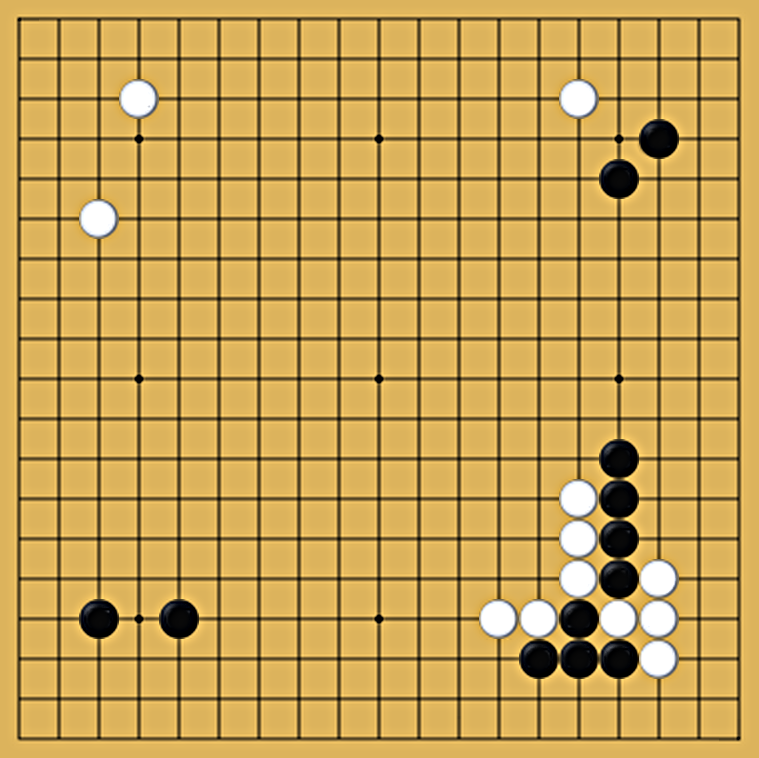
\includegraphics[width=\columnwidth]{images/ear-reddening-24.png}}%
				\only<2>{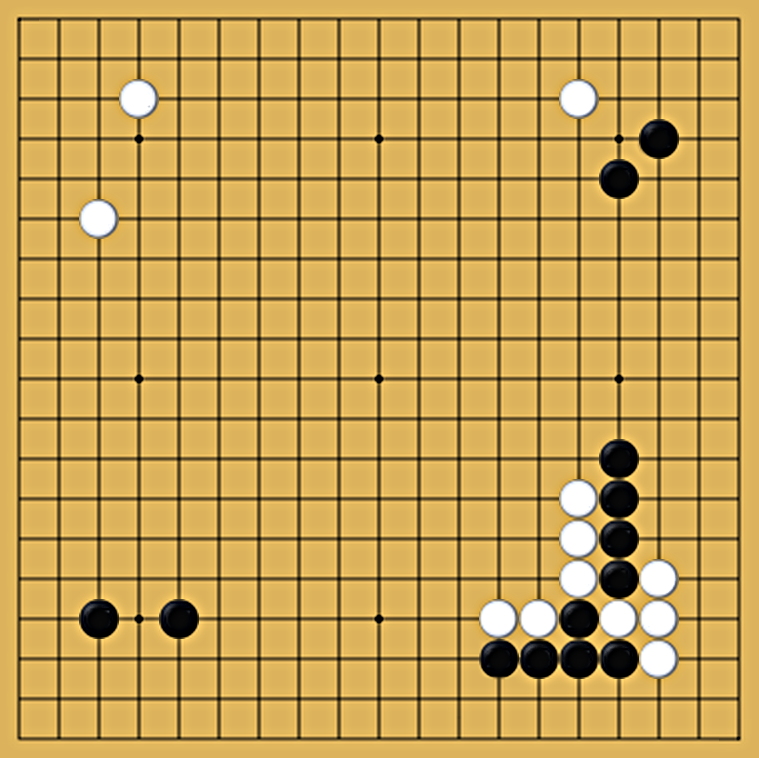
\includegraphics[width=\columnwidth]{images/ear-reddening-25.png}}%
				\only<3>{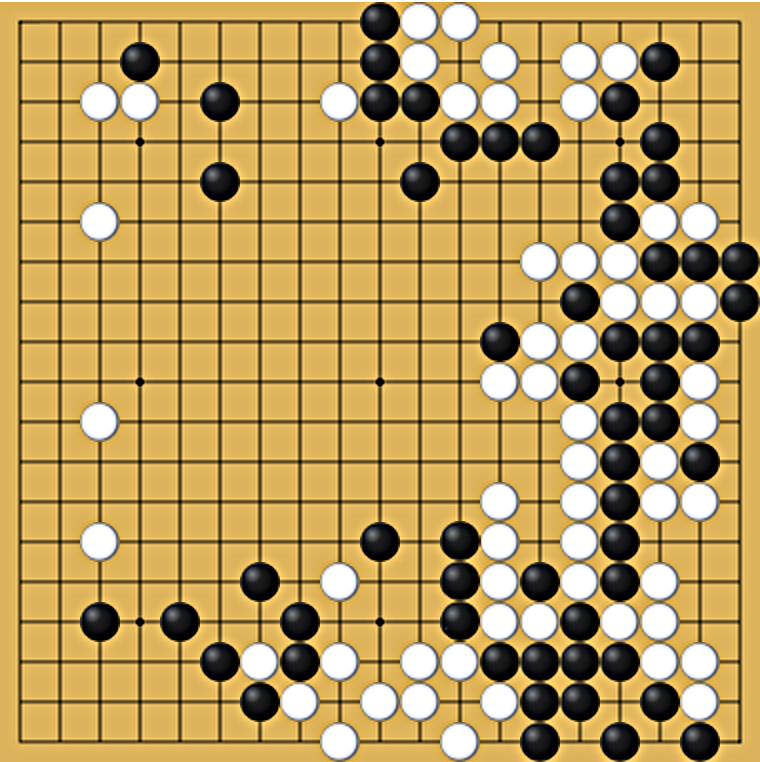
\includegraphics[width=\columnwidth]{images/ear-reddening-126.png}}%
				\only<4>{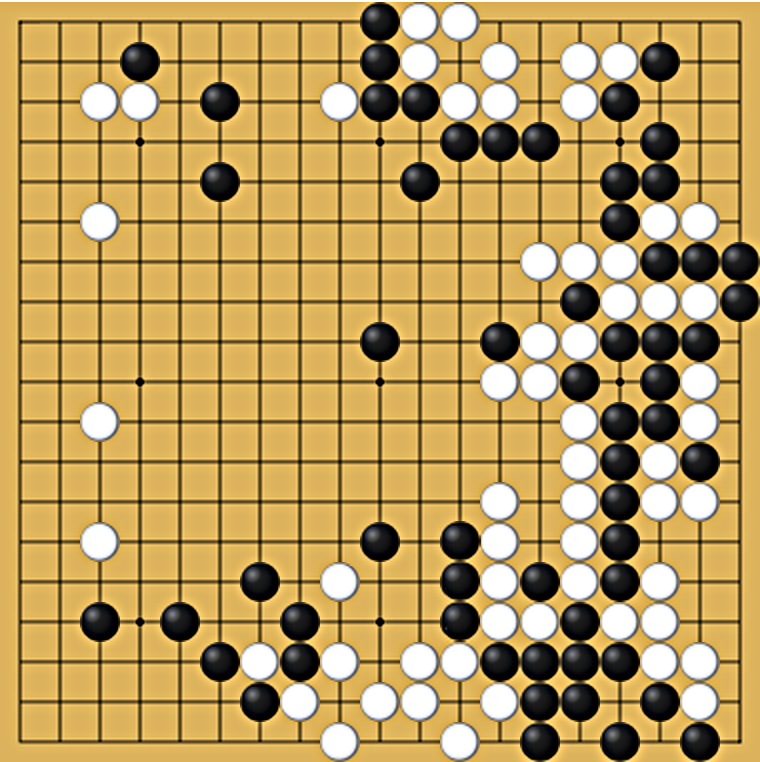
\includegraphics[width=\columnwidth]{images/ear-reddening-127.png}}%
				\caption{\tiny{Image CC-BY-SA 3.0 by Wikipedia \url{http://en.wikipedia.org/w/index.php?title=Ear-reddening_game&oldid=640966258}}}
			\end{figure}
		\end{column}
	\end{columns}
\end{frame}

\section{Detector Pipeline}
\frame[squeeze]{\tableofcontents[currentsection]}

\subsection{Overview}
\begin{frame}{Overview}
	Most of the related work uses only line detection to find the board \\
	$\Rightarrow$ This is problematic for mobile applications\\[0.5cm]

	Our approach is to \begin{itemize}
		\item use line detection for finding intersections
		\item detect pieces, too, for intersections
		\item extrapolate the board from both
		\item classify intersections
	\end{itemize}
\end{frame}

\subsection{Preprocessing}
\begin{frame}{Preprocessing}{Segmenting the board from the background}
	\begin{columns}
		\begin{column}{0.5\textwidth}
			Segmenting the board from the background is useful for
			\begin{itemize}
				\item removal of noisy backgrounds
				\item improving detection speed
			\end{itemize}
			\vspace{0.5cm}
			We use an adaptive threshold and connected-component analysis for this task
		\end{column}

		\begin{column}{0.45\textwidth}
			\only<1>{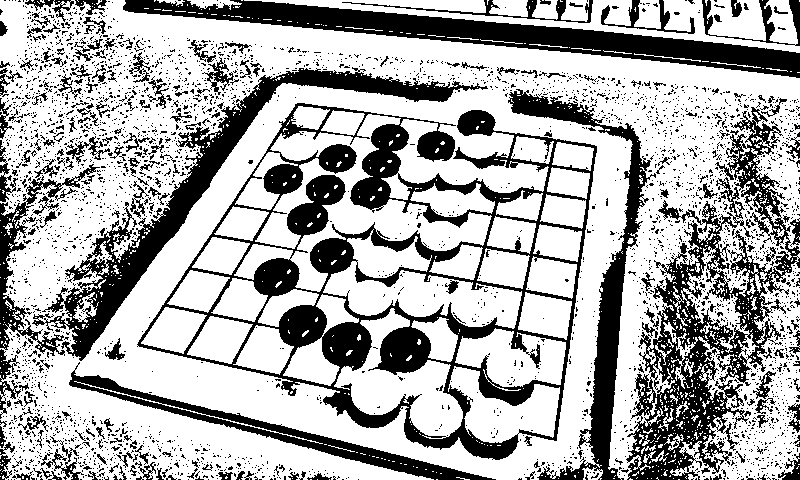
\includegraphics[width=\columnwidth]{images/prep_threshold.png}}%
			\only<2>{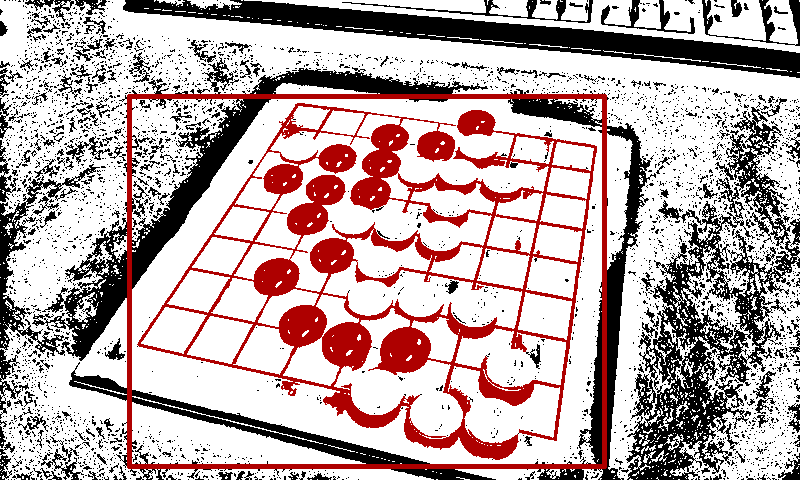
\includegraphics[width=\columnwidth]{images/prep_threshold_1.png}}%
			\only<3>{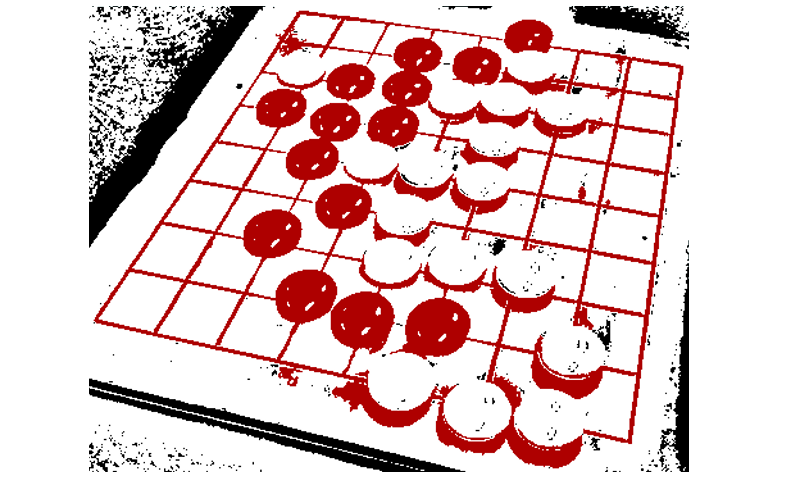
\includegraphics[width=\columnwidth]{images/prep_threshold_2.png}}
		\end{column}
	\end{columns}
\end{frame}

\subsection{Detection of Lines and Pieces}
\begin{frame}{Detection of Lines}{using Hough Lines Transformation}
	\begin{columns}
		\begin{column}{0.5\textwidth}
			This approach is pretty straight forward:
			\begin{itemize}
				\item detect lines
				\item classify as horizontal/vertical
				\item intersect each horizontal with each vertical
				\item remove duplicates
			\end{itemize}
		\end{column}

		\begin{column}{0.45\textwidth}
			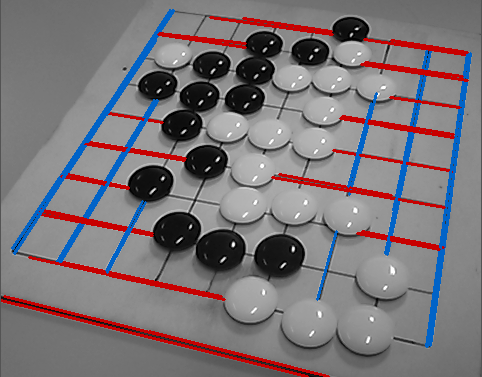
\includegraphics[width=\columnwidth]{images/lineDetection_hough.png}
		\end{column}
	\end{columns}
\end{frame}

\begin{frame}{Detection of Lines}{using the Line Segment Detector}
	\begin{columns}
		\begin{column}{0.45\textwidth}
			Additional steps for \emph{LSD} detector
			\begin{itemize}
				\item filter short lines
				\item filter lines without parallels
				\item stitch lines
			\end{itemize}
		\end{column}
		\begin{column}{0.5\textwidth}
			\begin{figure}
				\begin{center}
					\begin{subfigure}{}
						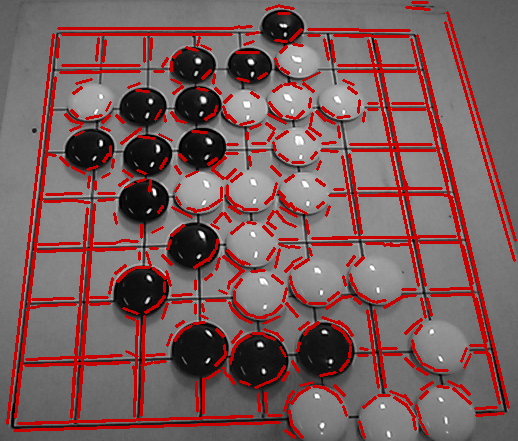
\includegraphics[width=0.45\columnwidth]{images/lsd_first.png}
					\end{subfigure}
					\begin{subfigure}{}
						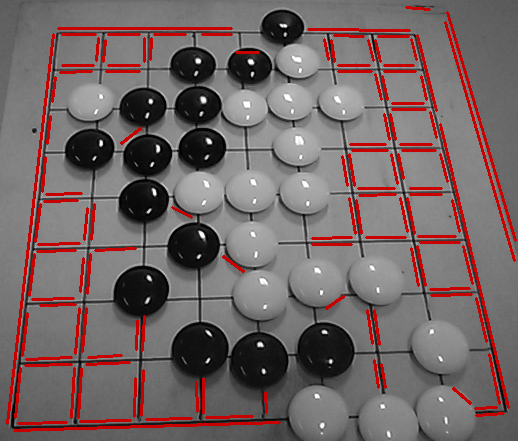
\includegraphics[width=0.45\columnwidth]{images/lsd_length.png}
					\end{subfigure}
					\\
					\begin{subfigure}{}
						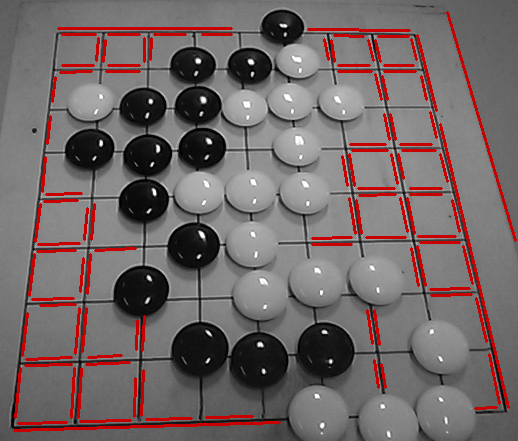
\includegraphics[width=0.45\columnwidth]{images/lsd_parallel.png}
					\end{subfigure}
					\begin{subfigure}{}
						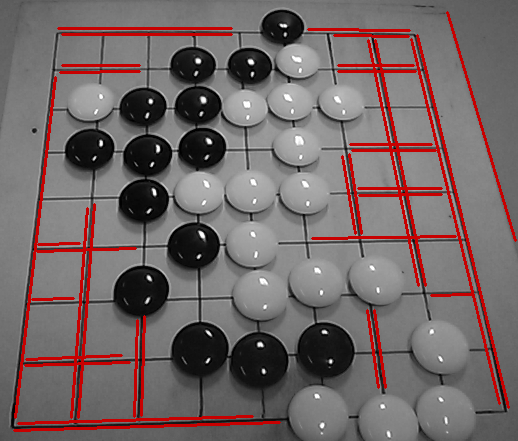
\includegraphics[width=0.45\columnwidth]{images/lsd_final.png}
					\end{subfigure}
				\end{center}
			\end{figure}
		\end{column}
	\end{columns}
\end{frame}

\begin{frame}{Detection of Pieces}{Thresholding}
	\begin{columns}
		\begin{column}{0.6\textwidth}
			To segment the tokens from the background we use thresholding\\[0.5cm]

			White pieces are a problem due to color aberration\\
			$\Rightarrow$ Threshold in HSV space, use combined results from saturation and hue channel\\[0.5cm]

			To detect the pieces we use \emph{Hough Transformation} or fit rectangles around the blobs and filter for squares
		\end{column}
		\begin{column}{0.3\textwidth}
			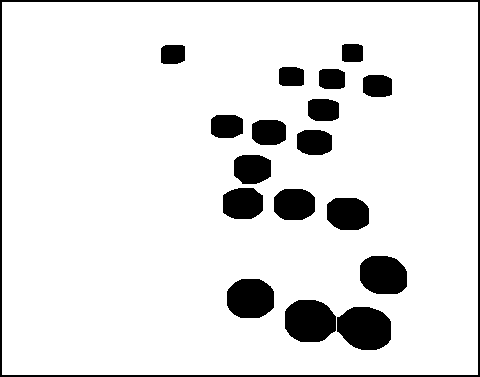
\includegraphics[width=\columnwidth]{images/pieces_thresh_s.png}\\
			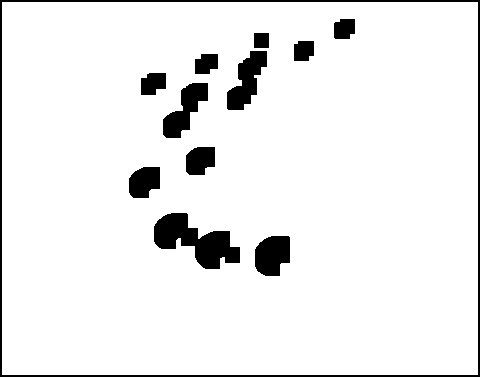
\includegraphics[width=\columnwidth]{images/pieces_thresh_v.png}
		\end{column}
	\end{columns}
\end{frame}
% \begin{frame}{Detection of Pieces}{using Hough Circle Transformation}~\end{frame}
% \begin{frame}{Detection of Pieces}{using contours of pieces}~\end{frame}

\subsection{Extrapolating the Board}
\begin{frame}{Extrapolating the Board}
	\begin{columns}
		\begin{column}{0.6\textwidth}
			We finally fill the intersections by
			\begin{itemize}
				\item rotating intersections to be horizontal
				\item selecting 20 around the center
				\item building a model from them
				\item detecting orientation of model with RANSAC
				\item using orientation to extrapolate board
				\item using detected intersections to refine extrapolation
			\end{itemize}
		\end{column}
		\begin{column}{0.3\textwidth}
			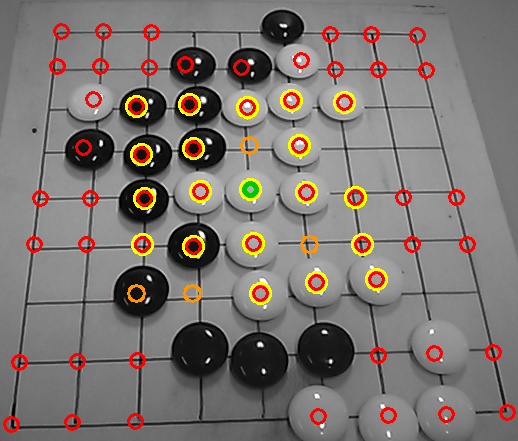
\includegraphics[width=\columnwidth]{images/buildingModel.png}\\
			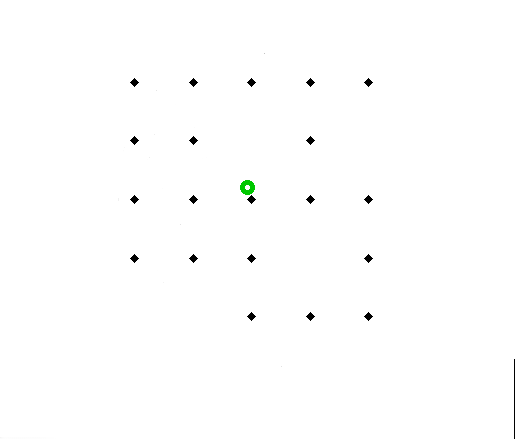
\includegraphics[width=\columnwidth]{images/builtModel.png}
		\end{column}
	\end{columns}
\end{frame}
\subsection{Postprocessing}
\begin{frame}{Postprocessing}
	We try to filter out invalid detection results. We consider results invalid if one intersection is
	\begin{itemize}
		\item outside the image
		\item or closer than 5px to each other.
	\end{itemize}
	\vspace{0.5cm}

	We undo the cropping from the preprocessing step.\\[0.5cm]

	We smooth results over time: only if a token was detected in 5 of the last 10 frames we count it as accurate.
\end{frame}

\section{Evaluation}
\frame[squeeze]{\tableofcontents[currentsection]}
\subsection{Image Set}
\begin{frame}{Image Set}
	\begin{itemize}
		\item We took 101 photos with different lighting and backgrounds
		\item 70 were used for empirical parameter optimization; 31 for testing
	\end{itemize}

	\begin{figure}
		\begin{subfigure}{}
			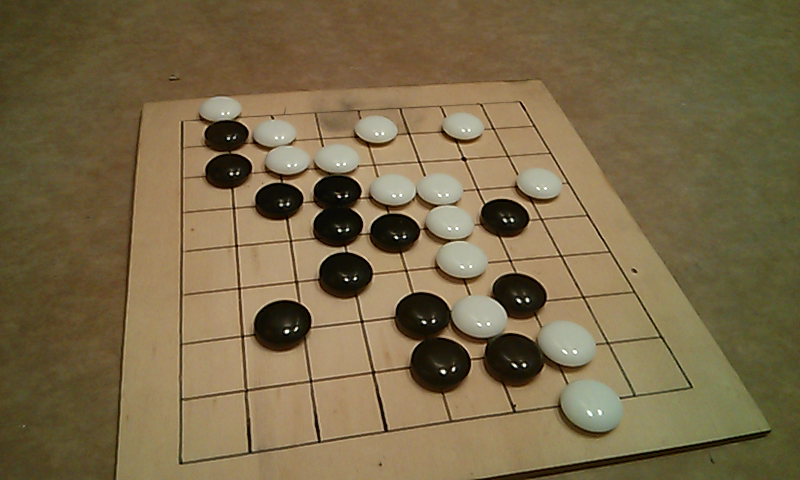
\includegraphics[width=0.3\columnwidth]{images/warmLight_many_leftMedium.png}
		\end{subfigure}
		~
		\begin{subfigure}{}
				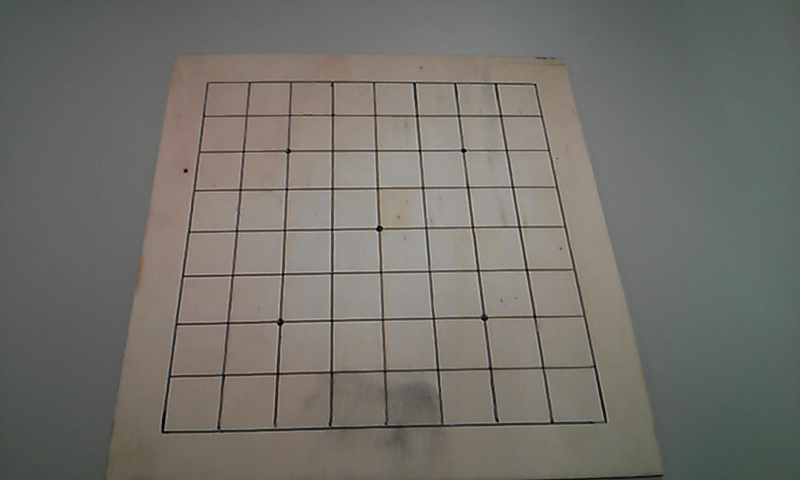
\includegraphics[width=0.3\columnwidth]{images/neonDesk_empty_centerAbove.png}
		\end{subfigure}
		~
		\begin{subfigure}{}
				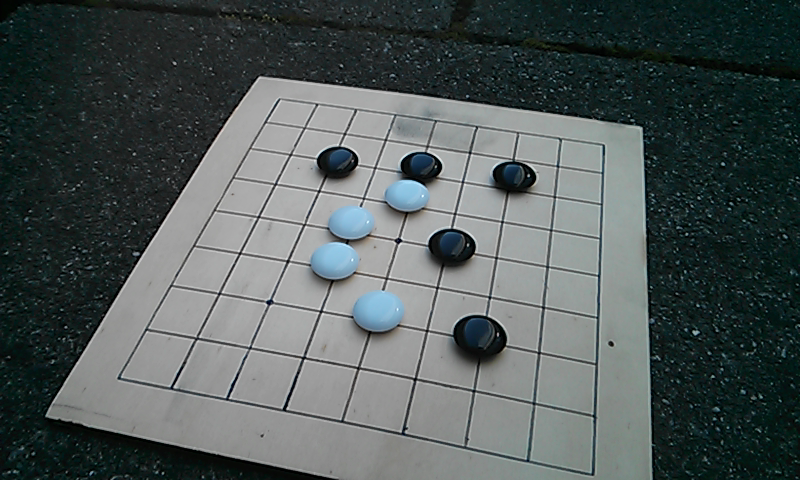
\includegraphics[width=0.3\columnwidth]{images/shadowStone_some_rightAbove.png}
		\end{subfigure}
		\\
		\begin{subfigure}{}
				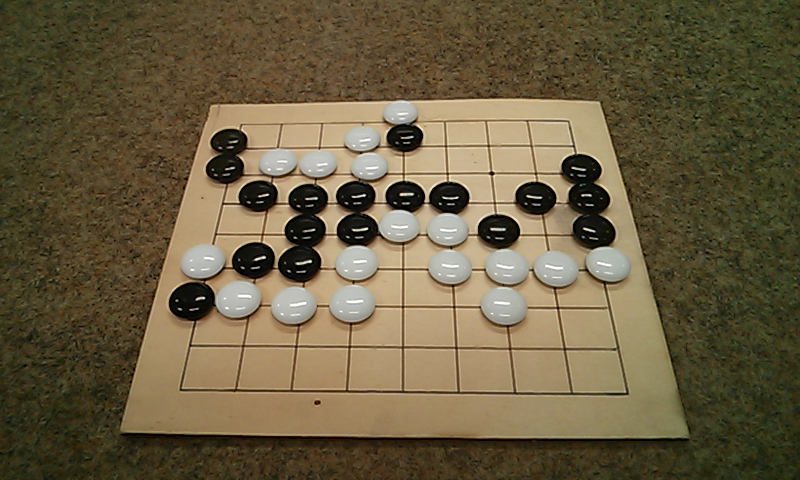
\includegraphics[width=0.3\columnwidth]{images/neonFloor_many_centerLow.png}
		\end{subfigure}
		~
		\begin{subfigure}{}
				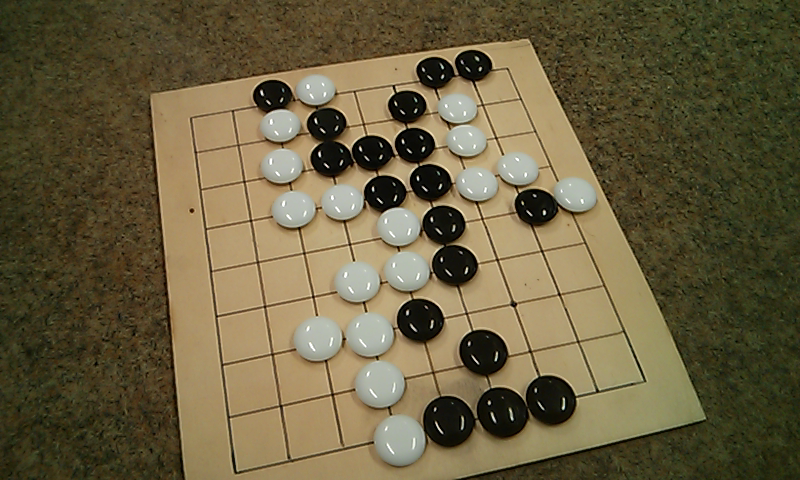
\includegraphics[width=0.3\columnwidth]{images/neonFloor_many_centerLow_rotated.png}
		\end{subfigure}
		~
		\begin{subfigure}{}
			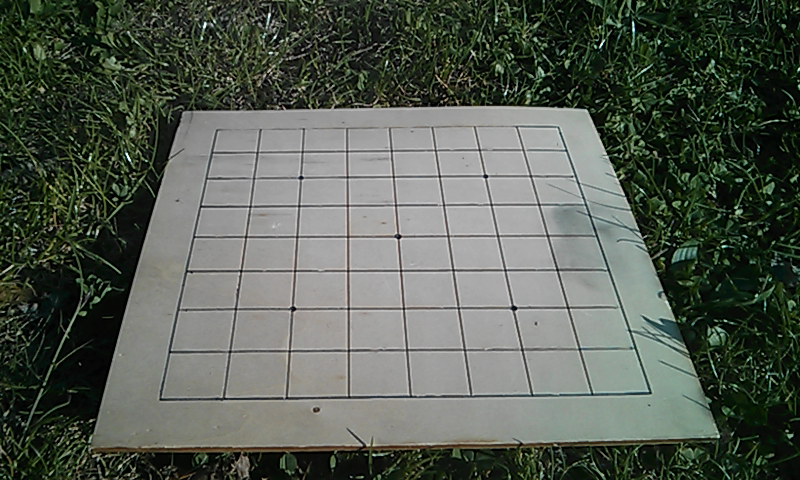
\includegraphics[width=0.3\columnwidth]{images/sunnyGrass_empty_centerLow.png}
		\end{subfigure}
	\end{figure}

\end{frame}

\subsection{Detection Quality}
\begin{frame}{Detection Quality}{Line detection algorithms}
	\begin{table}
		\centering
		\begin{tabular}{llc>{\bfseries}ccc}
		    \multicolumn{2}{c}{}									&\hphantom{A} & Hough 	& LSD 		& FAST     \\

			\toprule
			Empty board 			   		& Sensitivity 			&& 100\%	& 30.3\%  	& 0.685\%  \\
			%
											& Precision			 	&& 99.4\% 	& 94.2\%  	& 83.3\%  \\
			%																					  245/260	  5/6
			\midrule
			Some pieces (7-13)				& Sensitivity	 		&& 95.6\% 	& 11.4\% 	& 1.97\%   \\
			%
											& Precision 			&& 98.6\% 	& 91.2\%  	& 53.3\%  \\
			%																					  114/125	  16/30
			\midrule
			Many pieces (27-34) 			& Sensitivity		 	&& 58.6\% 	& 9.02\% 	& 3.80\%   \\
			%
											& Precision			 	&& 95.5\% 	& 94.0\%  	& 68.8\%  \\
			%																					  95/101	  33/48
			\bottomrule
		\end{tabular}
	\end{table}
	Sensitivity and precision on our test set. We evaluated correct ($\leq 15\text{px}$ off) intersections.
\end{frame}

\begin{frame}{Detection Quality}{Line detection algorithms}
	\vspace{-15pt}
	%!TEX root = Vortrag.tex

\begin{figure}
	\pgfplotsset{width=0.38\textwidth, height=5cm, compat=1.11}
	\pgfplotsset{every tick label/.append style={font=\tiny}}
	\pgfplotsset{every axis label/.append style={font=\tiny}}
	\pgfplotsset{every non boxed y axis/.append style={y axis line style=-}}
	\begin{subfigure}{}
		\begin{tikzpicture}
			\begin{axis}[
				xticklabels={,,},
				ylabel={Sensitivity \& Precision},
				xlabel={Tokens on the board},
				axis x line=bottom,
				axis y line=left,
				xmin=0,
				ymin=0,
				xmax=32,
				ymax=1
				]
				\draw[gray] ({rel axis cs:1,0}|-{axis cs:0,81}) -- ({rel axis cs:0,0}|-{axis cs:0,81});

				\addplot[only marks, mark=*, mark options={scale=1.1, fill=red!40!black}]
					table[x expr=\coordindex+1, y expr=\thisrow{matched}/(\thisrow{matched}+\thisrow{wrong})] {plots/lines_hough_testSet.csv};
				\addplot[only marks, mark=*, mark options={scale=1.1, fill=red}]
					table[x expr=\coordindex+1, y expr=\thisrow{matched}/81] {plots/lines_hough_testSet.csv};
			\end{axis}
		\end{tikzpicture}
	\end{subfigure}
	\begin{subfigure}{}
		\begin{tikzpicture}
			\begin{axis}[
				xticklabels={,,},
				xlabel={Tokens on the board},
				axis x line=bottom,
				axis y line=left,
				xmin=0,
				ymin=0,
				xmax=32,
				ymax=1
				]
				\draw[gray] ({rel axis cs:1,0}|-{axis cs:0,81}) -- ({rel axis cs:0,0}|-{axis cs:0,81});

				\addplot[only marks, mark=*, mark options={scale=1.1, fill=blue!40!black}]
					table[x expr=\coordindex+1, y expr=\thisrow{matched}/(\thisrow{matched}+\thisrow{wrong})] {plots/lines_lsd_testSet.csv};
				\addplot[only marks, mark=*, mark options={scale=1.1, fill=blue}]
					table[x expr=\coordindex+1, y expr=\thisrow{matched}/81] {plots/lines_lsd_testSet.csv};
			\end{axis}
		\end{tikzpicture}
	\end{subfigure}
	\begin{subfigure}{}
		\begin{tikzpicture}
			\begin{axis}[
				xticklabels={,,},
				xlabel={Tokens on the board},
				axis x line=bottom,
				axis y line=left,
				xmin=0,
				ymin=0,
				xmax=32,
				ymax=1
				]
				\draw[gray] ({rel axis cs:1,0}|-{axis cs:0,81}) -- ({rel axis cs:0,0}|-{axis cs:0,81});

				\addplot[only marks, mark=*, mark options={scale=1.1, fill=green!40!black}]
					table[x expr=\coordindex+1, y expr=\thisrow{matched}/(\thisrow{matched}+\thisrow{wrong})] {plots/intersections_fast_testSet.csv};
				\addplot[only marks, mark=*, mark options={scale=1.1, fill=green}]
					table[x expr=\coordindex+1, y expr=\thisrow{matched}/81] {plots/intersections_fast_testSet.csv};
			\end{axis}
		\end{tikzpicture}
	\end{subfigure}
\end{figure}

	\vspace{-15pt}
	Sensitivity (light color filled circles) and precision (dark color filled circles) per image in our test set.
\end{frame}

\begin{frame}{Detection Quality}{Piece detection algorithms}
	\vspace{-10pt}
	\begin{table}
		\centering
		\begin{tabular}{ll ccc}
		    \multicolumn{2}{c}{}											&\hphantom{A} & Contour 	& HOUGH	\\
			\toprule
			No pieces 								   		& Sensitivity 	&& N/A 				& N/A  			\\
															& Precision		&& 1 false positive & \bf{N/A} 		\\
			\midrule
			Some pieces (7-13)								& Sensitivity 	&& \bf{86.7\%} 	& 75.90\%			\\
			%												  72/83 		  63/83
															& Precision 	&& 98.6\% 		& \bf{100\%}		\\
			%												  72/73 		  63/63
			\midrule
			Many pieces (27-34) 							& Sensitivity 	&& 40.0\% 		& \bf{70.6\%} 		\\
			%												  243/357		  252/357
															& Precision		&& 99.2\% 		& 99.2\%			\\
			%												  246/248 		  252/254
			\specialrule{\heavyrulewidth}{\aboverulesep}{7pt}

			Total				 							& Sensitivity 	&& 71.6\% 		& 71.6\% 			\\
			%												  315/440		  315/440
															& Precision		&& 97.8\% 		& \textbf{99.3}\% 	\\
			%												  315/322 		  315/317
			\bottomrule
		\end{tabular}
	\end{table}
	Sensitivity and precision on our test set. We evaluated correct ($\leq 15\text{px}$ off) piece location and roughly correct piece size.
\end{frame}

\begin{frame}{Detection Quality}{Piece detection algorithms}
	\vspace{-15pt}
	%!TEX root = Vortrag.tex

\begin{figure}
	\centering
	\pgfplotsset{width=0.45\textwidth, height=5cm, compat=1.11}
	\pgfplotsset{every tick label/.append style={font=\tiny}}
	\pgfplotsset{every axis label/.append style={font=\tiny}}
	\pgfplotsset{every non boxed y axis/.append style={y axis line style=-}}
	\begin{subfigure}{}
		\begin{tikzpicture}
			\begin{axis}[
				xticklabels={,,},
				axis x line=bottom,
				axis y line=left,
				ylabel={Sensitivity \& Precision},
				xlabel={Tokens on the board},
				xmin=0,
				ymin=0,
				xmax=32,
				ymax=1
				]
				\draw[gray] ({rel axis cs:1,0}|-{axis cs:0,81}) -- ({rel axis cs:0,0}|-{axis cs:0,81});

				\addplot[only marks, mark=*, mark options={scale=1.1, fill=orange!40!black}]
					table[x expr=\coordindex+1, y expr=\thisrow{matched}/(\thisrow{matched}+\thisrow{wrong})] {plots/pieces_contour_testSet.csv};
				\addplot[only marks, mark=*, mark options={scale=1.1, fill=orange}]
					table[x expr=\coordindex+1, y expr=\thisrow{matched}/\thisrow{available}] {plots/pieces_contour_testSet.csv};
			\end{axis}
		\end{tikzpicture}
	\end{subfigure}
	\begin{subfigure}{}
		\begin{tikzpicture}
			\begin{axis}[
				xticklabels={,,},
				axis x line=bottom,
				axis y line=left,
				xlabel={Tokens on the board},
				xmin=0,
				ymin=0,
				xmax=32,
				ymax=1
				]
				\draw[gray] ({rel axis cs:1,0}|-{axis cs:0,81}) -- ({rel axis cs:0,0}|-{axis cs:0,81});

				\addplot[only marks, mark=*, mark options={scale=1.1, fill=magenta!40!black}]
					table[x expr=\coordindex+1, y expr=\thisrow{matched}/(\thisrow{matched}+\thisrow{wrong})] {plots/pieces_hough_testSet.csv};
				\addplot[only marks, mark=*, mark options={scale=1.1, fill=magenta}]
					table[x expr=\coordindex+1, y expr=\thisrow{matched}/\thisrow{available}] {plots/pieces_hough_testSet.csv};
			\end{axis}
		\end{tikzpicture}
	\end{subfigure}
\end{figure}

	\vspace{-15pt}
	Sensitivity (light color filled circles) and precision (dark color filled circles) per image in our test set.
\end{frame}

\subsection{Speed}
\definecolor{rosso}{RGB}{220,57,18}
\definecolor{giallo}{RGB}{255,153,0}
\definecolor{blu}{RGB}{102,140,217}
\definecolor{verde}{RGB}{16,150,24}
\definecolor{viola}{RGB}{153,0,153}

\makeatletter

\tikzstyle{chart}=[
    legend label/.style={font={\scriptsize},anchor=west,align=left},
    legend box/.style={rectangle, draw, minimum size=5pt},
    axis/.style={black,semithick,->},
    axis label/.style={anchor=east,font={\tiny}},
]

\tikzstyle{bar chart}=[
    chart,
    bar width/.code={
        \pgfmathparse{##1/2}
        \global\let\bar@w\pgfmathresult
    },
    bar/.style={very thick, draw=white},
    bar label/.style={font={\bf\small},anchor=north},
    bar value/.style={font={\footnotesize}},
    bar width=.75,
]

\tikzstyle{pie chart}=[
    chart,
    slice/.style={line cap=round, line join=round, very thick,draw=white},
    pie title/.style={font={\bf}},
    slice type/.style 2 args={
        ##1/.style={fill=##2},
        values of ##1/.style={}
    }
]

\pgfdeclarelayer{background}
\pgfdeclarelayer{foreground}
\pgfsetlayers{background,main,foreground}


\newcommand{\pie}[3][]{
    \begin{scope}[#1]
    \pgfmathsetmacro{\curA}{90}
    \pgfmathsetmacro{\r}{1}
    \def\c{(0,0)}
    \foreach \v/\s in{#3}{
        \pgfmathsetmacro{\deltaA}{\v/100*360}
        \pgfmathsetmacro{\nextA}{\curA + \deltaA}
        \pgfmathsetmacro{\midA}{(\curA+\nextA)/2}

        \path[slice,\s] \c
            -- +(\curA:\r)
            arc (\curA:\nextA:\r)
            -- cycle;
        \pgfmathsetmacro{\d}{max((\deltaA * -(.5/50) + 1) , .5)}

        \begin{pgfonlayer}{foreground}
        \path \c -- node[pos=\d,pie values,values of \s]{} +(\midA:\r);
        \end{pgfonlayer}

        \global\let\curA\nextA
    }
    \end{scope}
}

\newcommand{\legend}[2][]{
    \begin{scope}[#1]
    \path
        \foreach \n/\s in {#2}
            {
                  ++(0,-10pt) node[\s,legend box] {} +(5pt,0) node[legend label] {\n}
            }
    ;
    \end{scope}
}

\begin{frame}[fragile]{Speed}
	\center
	\pgfplotstableread[header=false]{
		345.24 	{Hough lines}
		168.46	{LSD lines}
		322.58	{Hough pieces}
		249.69	{Contour pieces}
		208.04 {Preprocessing}
		83.16 {Extrapolate board}
		26.39 {Detect colors}
		51.33 {Framework}
		64.21 {Create output}
		}\datatable
		\pgfplotsset{
	    select row/.style={
	        x filter/.code={\ifnum\coordindex=#1\else\def\pgfmathresult{}\fi}
	    }
	}
	\begin{figure}
		\pgfplotsset{width=1.1\textwidth, height=6cm, compat=1.11}
		\begin{subfigure}{}
			\begin{tikzpicture}
				 \begin{axis}[
					        xbar,
					        bar shift=0pt,
					        xmin=0,
					        xmax=430,
					        width=0.8\textwidth,
					        ytick={0, 1, 2.5, 3.5, 5, 6, 7, 8, 9},
					        yticklabels from table={\datatable}{1},
					        ytick pos=left,
					        xmajorgrids = true,
					        xlabel={Time in ms},
					        width=0.74\textwidth,
					        nodes near coords, nodes near coords align={horizontal}
					  ]

					\addplot[fill=gray] table [select row=8, y expr=9] {\datatable}; %framework
					\addplot[fill=gray] table [select row=7, y expr=8] {\datatable}; %framework
					\addplot[fill=red!60!white] table [select row=6, y expr=7] {\datatable}; %color extraction
					\addplot[fill=blue!60!white] table [select row=5, y expr=6] {\datatable}; %extrapolate board
					\addplot[fill=green!80!black] table [select row=4, y expr=5] {\datatable}; %preprocessing
					\addplot[fill=orange] table [select row=3, y expr=3.5] {\datatable}; %contour pieces
					\addplot[fill=magenta] table [select row=2, y expr=2.5] {\datatable}; %hough pieces
					\addplot[fill=blue] table [select row=1, y expr=1] {\datatable}; %lsd
					\addplot[fill=red] table [select row=0, y expr=0] {\datatable}; %hough lines
				  \end{axis}
			\end{tikzpicture}
		\end{subfigure}
		% ~
		% \begin{subfigure}{}
		% 	\vspace{15pt}
		% 	\begin{tikzpicture}
		% 		[
		% 		    pie chart,
		% 		    slice type={preprocessing}{green!80!black},
		% 		    slice type={line detection}{red},
		% 		    slice type={piece detection}{orange},
		% 		    slice type={extrapolate board}{blue!60!white},
		% 		    slice type={color extraction}{red!60!white},
		% 		    slice type={framework}{gray},
		% 		    pie values/.style={font={\small}},
		% 		    scale=2
		% 		]
		% 	    \pie{}{
		%     			18.98/preprocessing,
		%     			31.5/{line detection},
		%     			22.78/{piece detection},
		%     			7.58/{extrapolate board},
		%     			2.41/{color extraction},
		%     			10.54/framework}

		% 	\end{tikzpicture}
		% 	\vspace{1.5em}
		% \end{subfigure}
	\end{figure}
	Average duration of parts of the pipeline over 100 iterations on a \emph{Nexus 4}
\end{frame}

\newcommand*\leftlap[2]{\hphantom{#1}\llap{#2}}
\newcommand*\rightlap[2]{\rlap{#2}\hphantom{#1}}
\begin{frame}{Overall Quality}{Accuracy of our final detector on our image sets}
	\begin{table}
	\center
		\begin{tabular}{rlccc}
			  &\	 		 			& 	Trainingset 	 && Testset 				\\
			\toprule
			Number of images			&&	70					 &&		31							\\
			Discarded results		 	&&	 5					 &&		 2							\\
			Accuracy localizing			&&	99.1\% (5217/5265)	 && \leftlap{98.6}{100}\% (2349/2349) \\
			Accuracy classifying		&&	98.0\% (5112/5217)	 && 98.6\% (2317/2349)				\\
			Accuracy for both			&&	97.1\% (5112/5265)	 && 98.6\% (2317/2349) 				\\
			\bottomrule
		\end{tabular}
	\end{table}
	\vfill
	Similar quality is shown in tests where real games were played and recorded.
\end{frame}

\section{Conclusion}
\subsection{Our Contribution}
\begin{frame}{Our Contribution}
	\begin{columns}
		\begin{column}{0.5\textwidth}
			\begin{itemize}
				\item We present a reliable method for the detection of Go boards
				\item Our method is fast enough to be used on smartphones
				\item We can detect boards with dense token distribution
				\item We showcase a possible approach for an end user product
			\end{itemize}
		\end{column}
		\begin{column}{0.4\textwidth}
			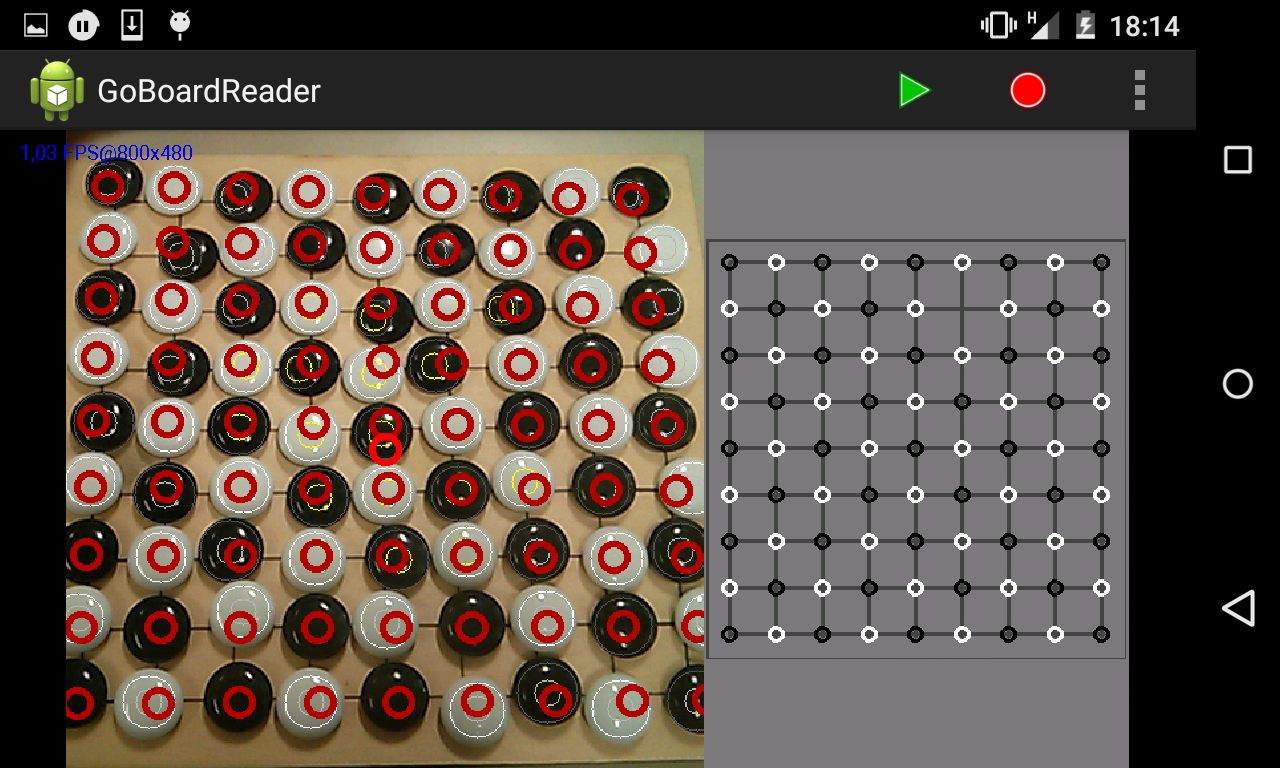
\includegraphics[width=\columnwidth]{images/android_perfect_recognition.png}
		\end{column}
	\end{columns}
\end{frame}
\subsection{Future Work}
\begin{frame}{Future Work}
	Possible areas of future work could be:
	\begin{itemize}
		\item extending the approach to a 19x19 grid or grids of arbitrary size
		\item autonomously detecting the center of the board
		\item improving correction of specular highlights
	\end{itemize}
\end{frame}

\subsection{Live Presentation}
\begin{frame}{Live presentation}{Because seeing is believing}
	\centering
	If there is still time...
\end{frame}

\section*{Questions}
\begin{frame}
	\centering
  \huge Thank you for your attention.\\[1.5cm] Questions?
\end{frame}

\end{document}
\endinput
%%
%% End of file `01-example'.
